\chapter{Pre-study} 


%Within the academic community, there exists a concerted effort to address issues related to energy efficiency and the adoption of renewable energy sources. 
%There are numerous research and ongoing projects aimed at establishing a robust social energy infrastructure capable of adapting to the utilisation of renewable energy sources. 
%Studies are also investigating the feasibility and practicalities of establishing zero-emission households and buildings.
%Technological innovations designed to support these goals have also been a focal point in the academic discourse surrounding energy efficiency and the transition to renewable energy.

%In the meantime, Palmer et al. \cite{informationgap} drew attention to the fact that engineering studies have identified various investments in new energy-efficient equipment or building retrofits that would generate savings surpassing their costs in terms of lower future energy expenses. However, homeowners and businesses lack sufficient knowledge and guidance on how to effectively utilize these opportunities to their advantage.

%Empirical results suggest that households' propensity to invest in clean energy technologies depends mainly on home ownership, income, social context and household energy conservation practices,
%in addition, environmental attitudes and beliefs, as manifest in energy conservation practices or membership in an environmental non-governmental organisation, also play a relevant role in technology adoption \cite{determinants}.

\section{Motivators for homeowners}

A comprehensive survey conducted by Palmer et al. \cite{informationgap} in the United States revealed various motivating factors that influence homeowners in their decision to investments in improving energy efficiency. 
Notably, saving money on utility bills (72\%) emerged as the primary motivator, 
closely followed by the low costs associated with improvements (66\%). 
These findings suggest that homeowners prioritise the financial aspects of energy efficiency when making retrofit and investment decisions. 
Surprisingly, preferences related to environmental sustainability ("Green") and the potential increase in property values do not appear to significantly influence their decisions.


\section{Social practices}

Currently, homeowners have limited avenues to access information about home energy systems. 
Presently, individuals seeking such information typically have two options. 
One is visiting the official websites of specific technology providers or physically visiting nearby stores that specialise in the sale of one or various energy technologies. 
However, this necessitates a prerequisite understanding of the particular energy technology.
Moreover, the information obtained through this approach may be restricted to the specific technology being explored, thus failing to offer a holistic perspective on the overall energy system, as energy technologies often function collaboratively.
An alternative approach is through professional home energy assessments, commonly known as home energy audits.
These assessments are conducted by experts who visit the house and perform a comprehensive inspection. 
Following the assessment, these professionals provide recommendations regarding house renovations, and in some cases, advice on suitable energy technologies to optimise energy efficiency.


\section{Research-based models}

Several research-based models furnish evidence to aid homeowners in making informed decisions regarding home energy systems.

\subsection{PVGIS online tool}
PVGIS \cite{pvgis} is a web-based application by the European Commission's Joint Research Centre, 
that enables users to access comprehensive data regarding solar radiation and the energy production of \gls{pv} systems. 
This service encompasses a wide range of geographical regions, including Europe, Africa, substantial portions of Asia, and America.
Which can be of a great help to house owners when deciding an investment in a \gls{pv} system. 

As shown in the Figure \ref{fig:pvgis}, the interactive tool allows users to navigate through the map and obtain information regarding performance of grid-connected \gls{pv} based on the selected location. 
The visualisation of monthly energy output provides a clear and descriptive representation of the energy generated by a \gls{pv} system throughout a year. 
Additionally, the outcome offers highly precise and specialised data, including detailed parameters such as yearly in-plane irradiation and year-to-year variability as well. 
While this information is highly valuable for researchers, it may pose comprehension challenges for homeowners lacking expertise in the field, thereby hindering their learning process. 
Furthermore, the data provided is only \gls{pv} related, lacking the connection to the specific circumstances of individual households. 
\begin{figure}[h!]
  \centering
  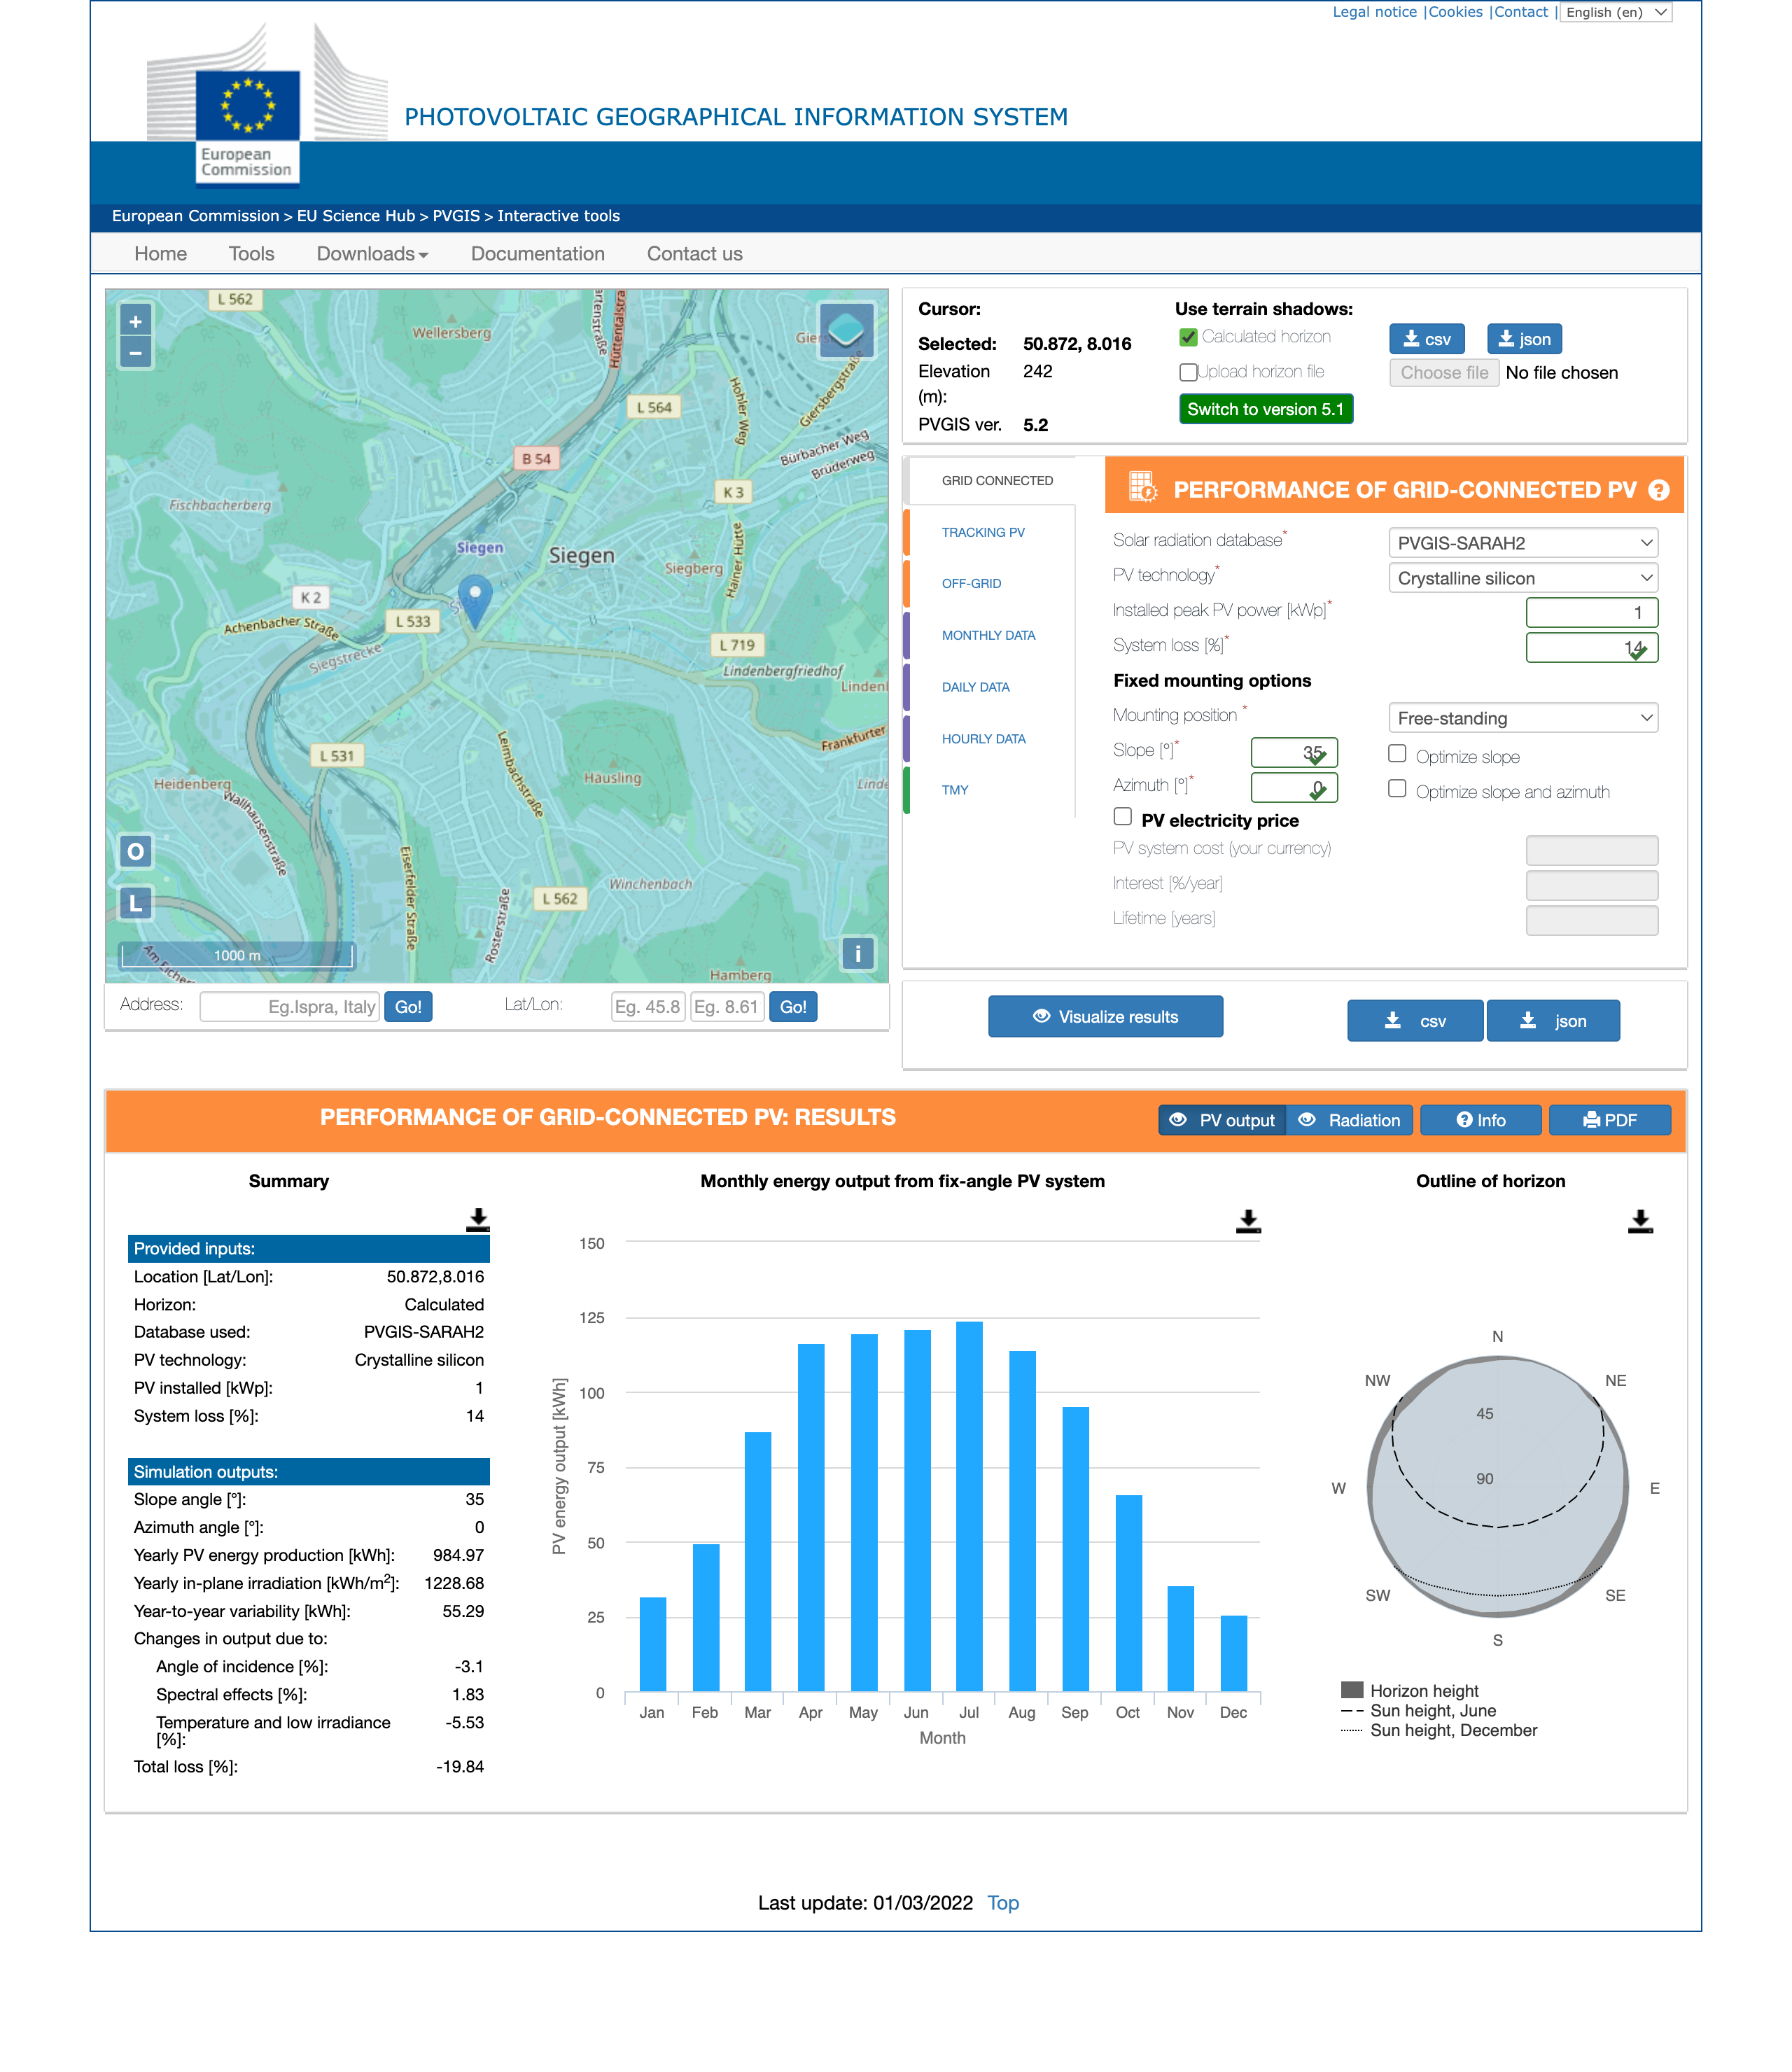
\includegraphics[width=\textwidth]{Images/pvgis.png}
  \caption{Screen of PVGIS online tool}
  \label{fig:pvgis}
\end{figure}

\subsection{FLEX models}

The FLEX models \cite{newtrends}, developed under the newTRENDs project\footnote{https://newtrends2020.eu/} by the Fraunhofer Institute for Systems and Innovation Research, 
are capable of calculating the energy demand of buildings at an hourly resolution. 
These models were developed to offer evidence-based information to decision-makers in industry, government, and civil society. 
%By providing a comprehensive assessment of the impacts of emerging technologies and innovation strategies, these models enable stakeholders to make informed decisions concerning policies related to technology and innovation. 

The models take various factors into account, including weather condition, household behaviours and energy technologies, as illustrated in Figure \ref{fig:flex-operation}.
Consequently, it offers a comprehensive evaluation of the energy consumption of a representative building. 
Moreover, the tool can be used to predict energy bills, enabling comparisons of energy expenses associated with different technology adoptions. 

%The Figure \ref{fig:flex} shows how FLEX interacts with other bottom-up models involved in the newTRENDs project,
%where FLEX-Operation and FLEX-Behaviour models are closely related to the demand and supply of energy for households. 
%\begin{figure}[h]
%  \centering
%  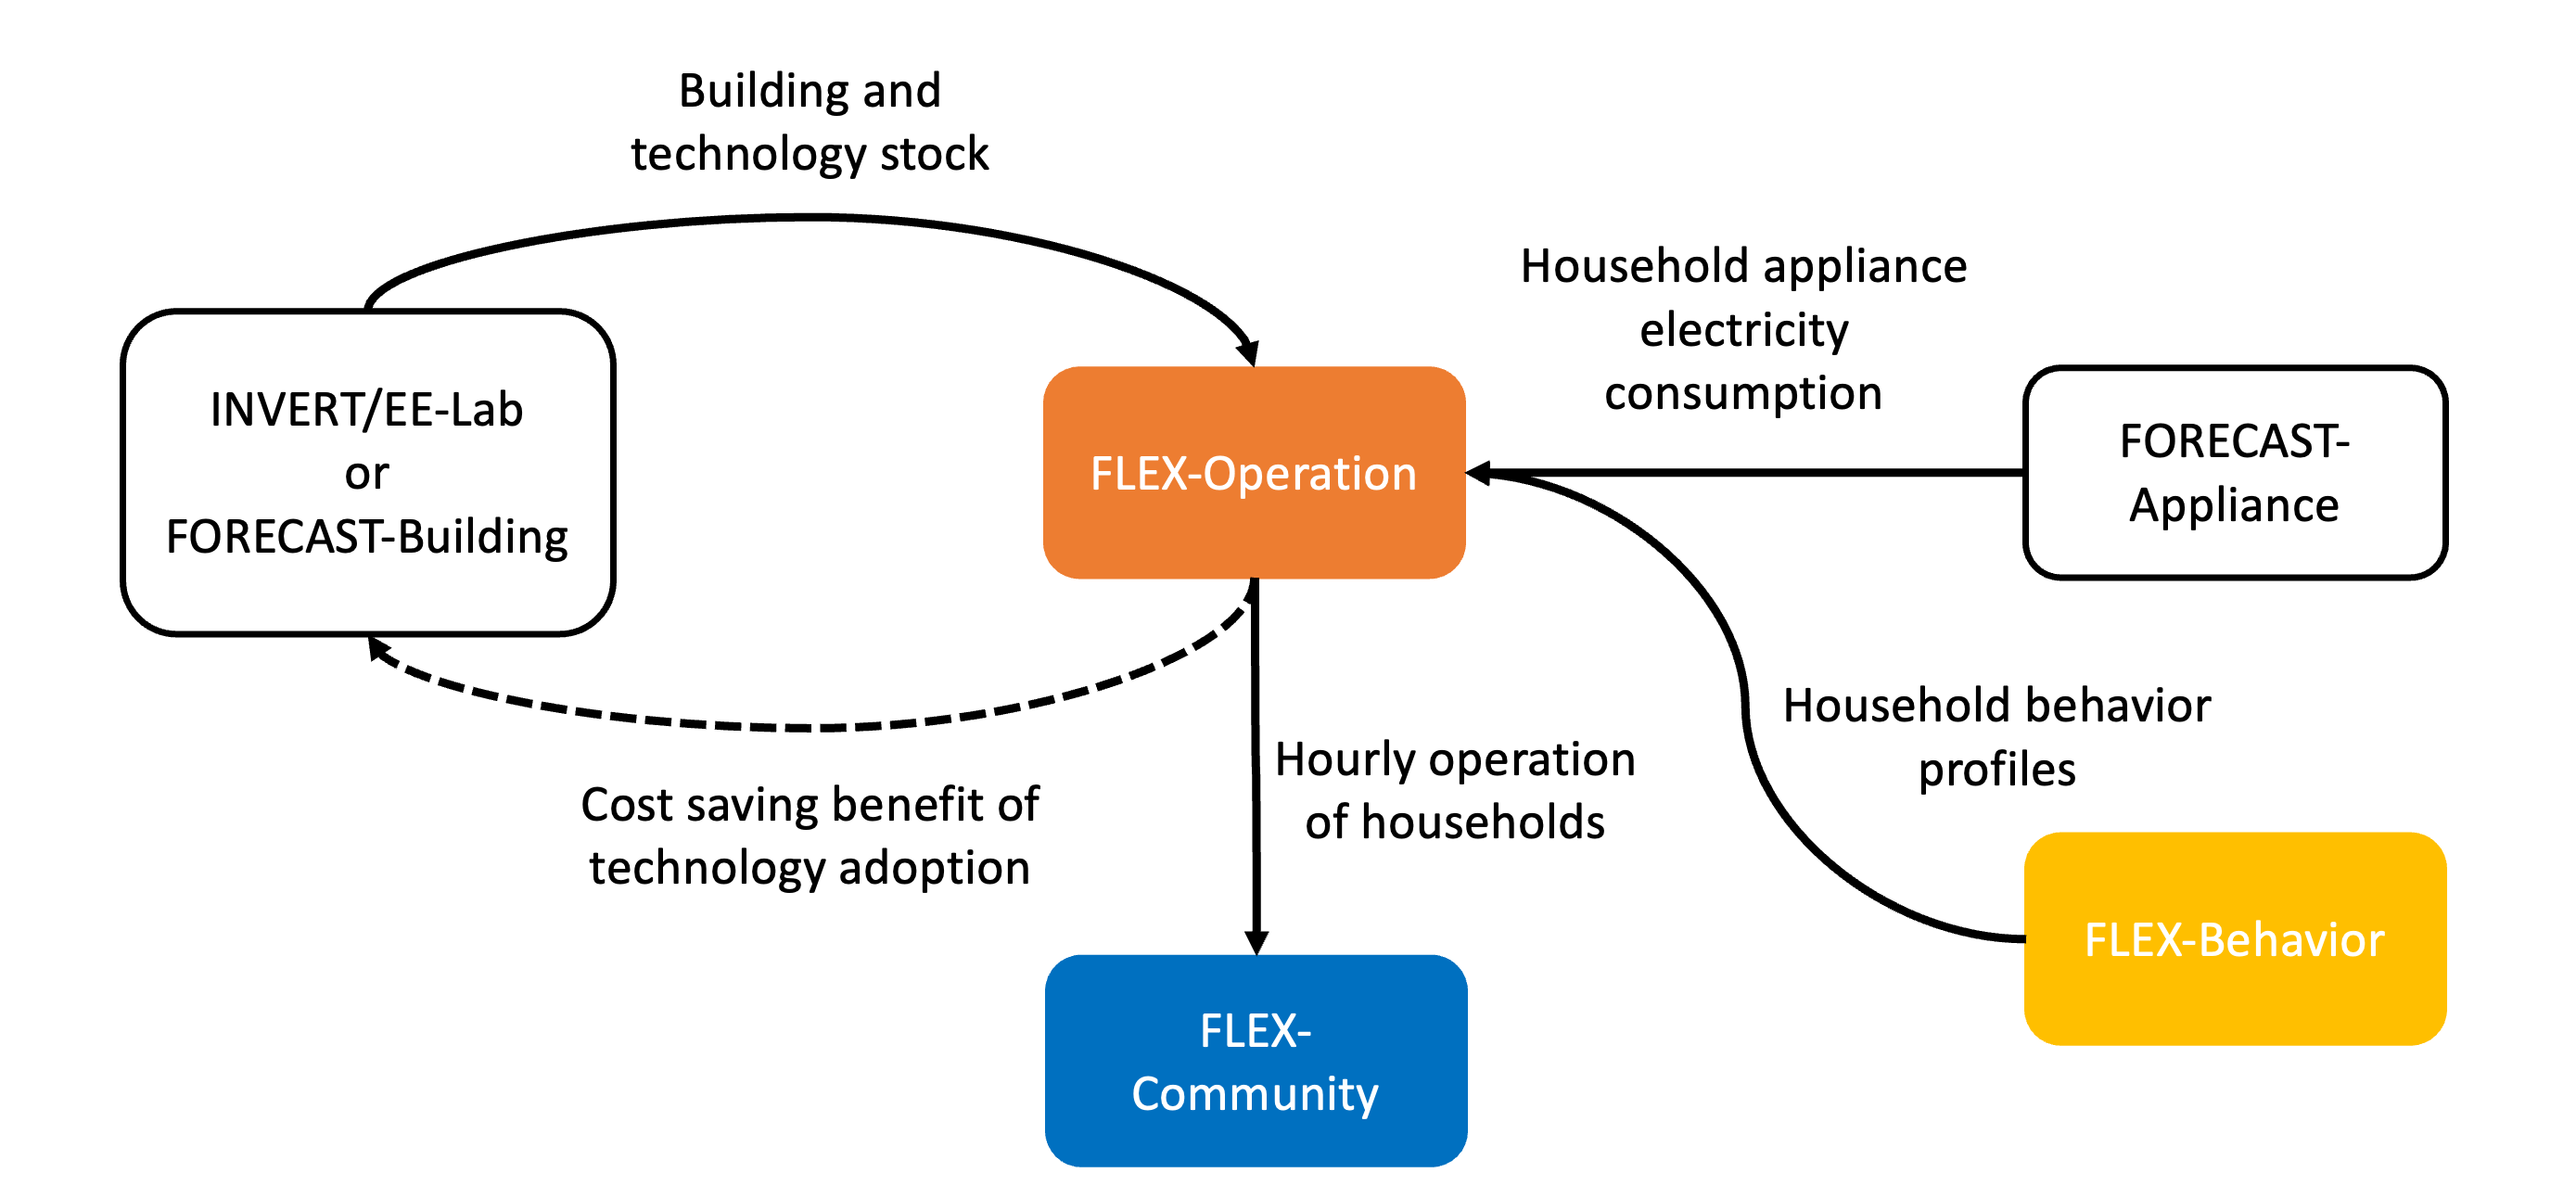
\includegraphics[width=\textwidth]{Images/flex.png}
%  \caption{FLEX modeling suite}
%  \label{fig:flex}
%\end{figure}

%Renewable energy (\gls{re}) and energy efficiency (\gls{ee}) are two central strategies pursued by the \gls{eu} and its Member States concerning the energy system. 
%In 2019, 80.9\% of our total energy supply still depended on burning fossil fuels, namely 26.8\% coal, 30.9\% oil and 23.2\% natural gas \cite{iea}. 
%Investments into low-carbon power generation accounted for 15\% recently are expected to rise to more than 30\% by 2030, corresponding to a quadrupling in absolute volumes \cite{shift}. Solar, wind, and the investments for enabling the integration of these technologies to the grid dominate the investments into low-carbon power generation \cite{shift}. 
%Electrification is playing a major role in the energy transition process. 
%Meanwhile, different electrification strategies rely heavily on energy efficiency \cite{electrification}.
%Measures to increase energy efficiency, including investments in energy savings and the consolidation of consultancy and information services, are promoted by The National Action Plan on Energy Efficiency (\gls{nape}) \cite{bafa}.  

%Transitioning towards a sustainable energy system necessitates significant effort on both the demand and supply sides. 
%However, previous research has shown that in many areas energy efficiency gains were counteracted by societal trends that increased corresponding activities, leading to much smaller decreases (or even increases) of energy demand than technologically feasible \cite{2050}. 
%The aim of newTRENDs is to increase the qualitative and quantitative understanding of impacts of new societal trends on energy consumption and to improve the modelling of energy demand, energy efficiency and policy instruments \cite{fraunhofer}. 


%\subsubsection{The FLEX-Operation model}

%The FLEX-Operation model \cite{newtrends} enables the detailed simulation of energy system operation for individual households at an hourly resolution. 
%This model provides a comprehensive assessment of the energy consumption of a representative building, incorporating technology operation (such as battery, \gls{pv}, and \gls{hp} systems) and load profiles at an hourly resolution. 
%In addition to its capability of modeling energy system operation, FLEX-Operation can also aid in investment decision-making by evaluating the energy-saving benefits associated with technology adoption.
%
%As shown in Figure \ref{fig:flex-operation}, FLEX-Operation considers following services:

%\begin{enumerate}
%  \item electric appliances, e.g., television, refrigerator, lighting, etc.;
%  \item space heating;
%  \item domestic hot water;
%  \item space cooling;
%  \item vehicle. 
%\end{enumerate}

\begin{figure}[h]
  \centering
  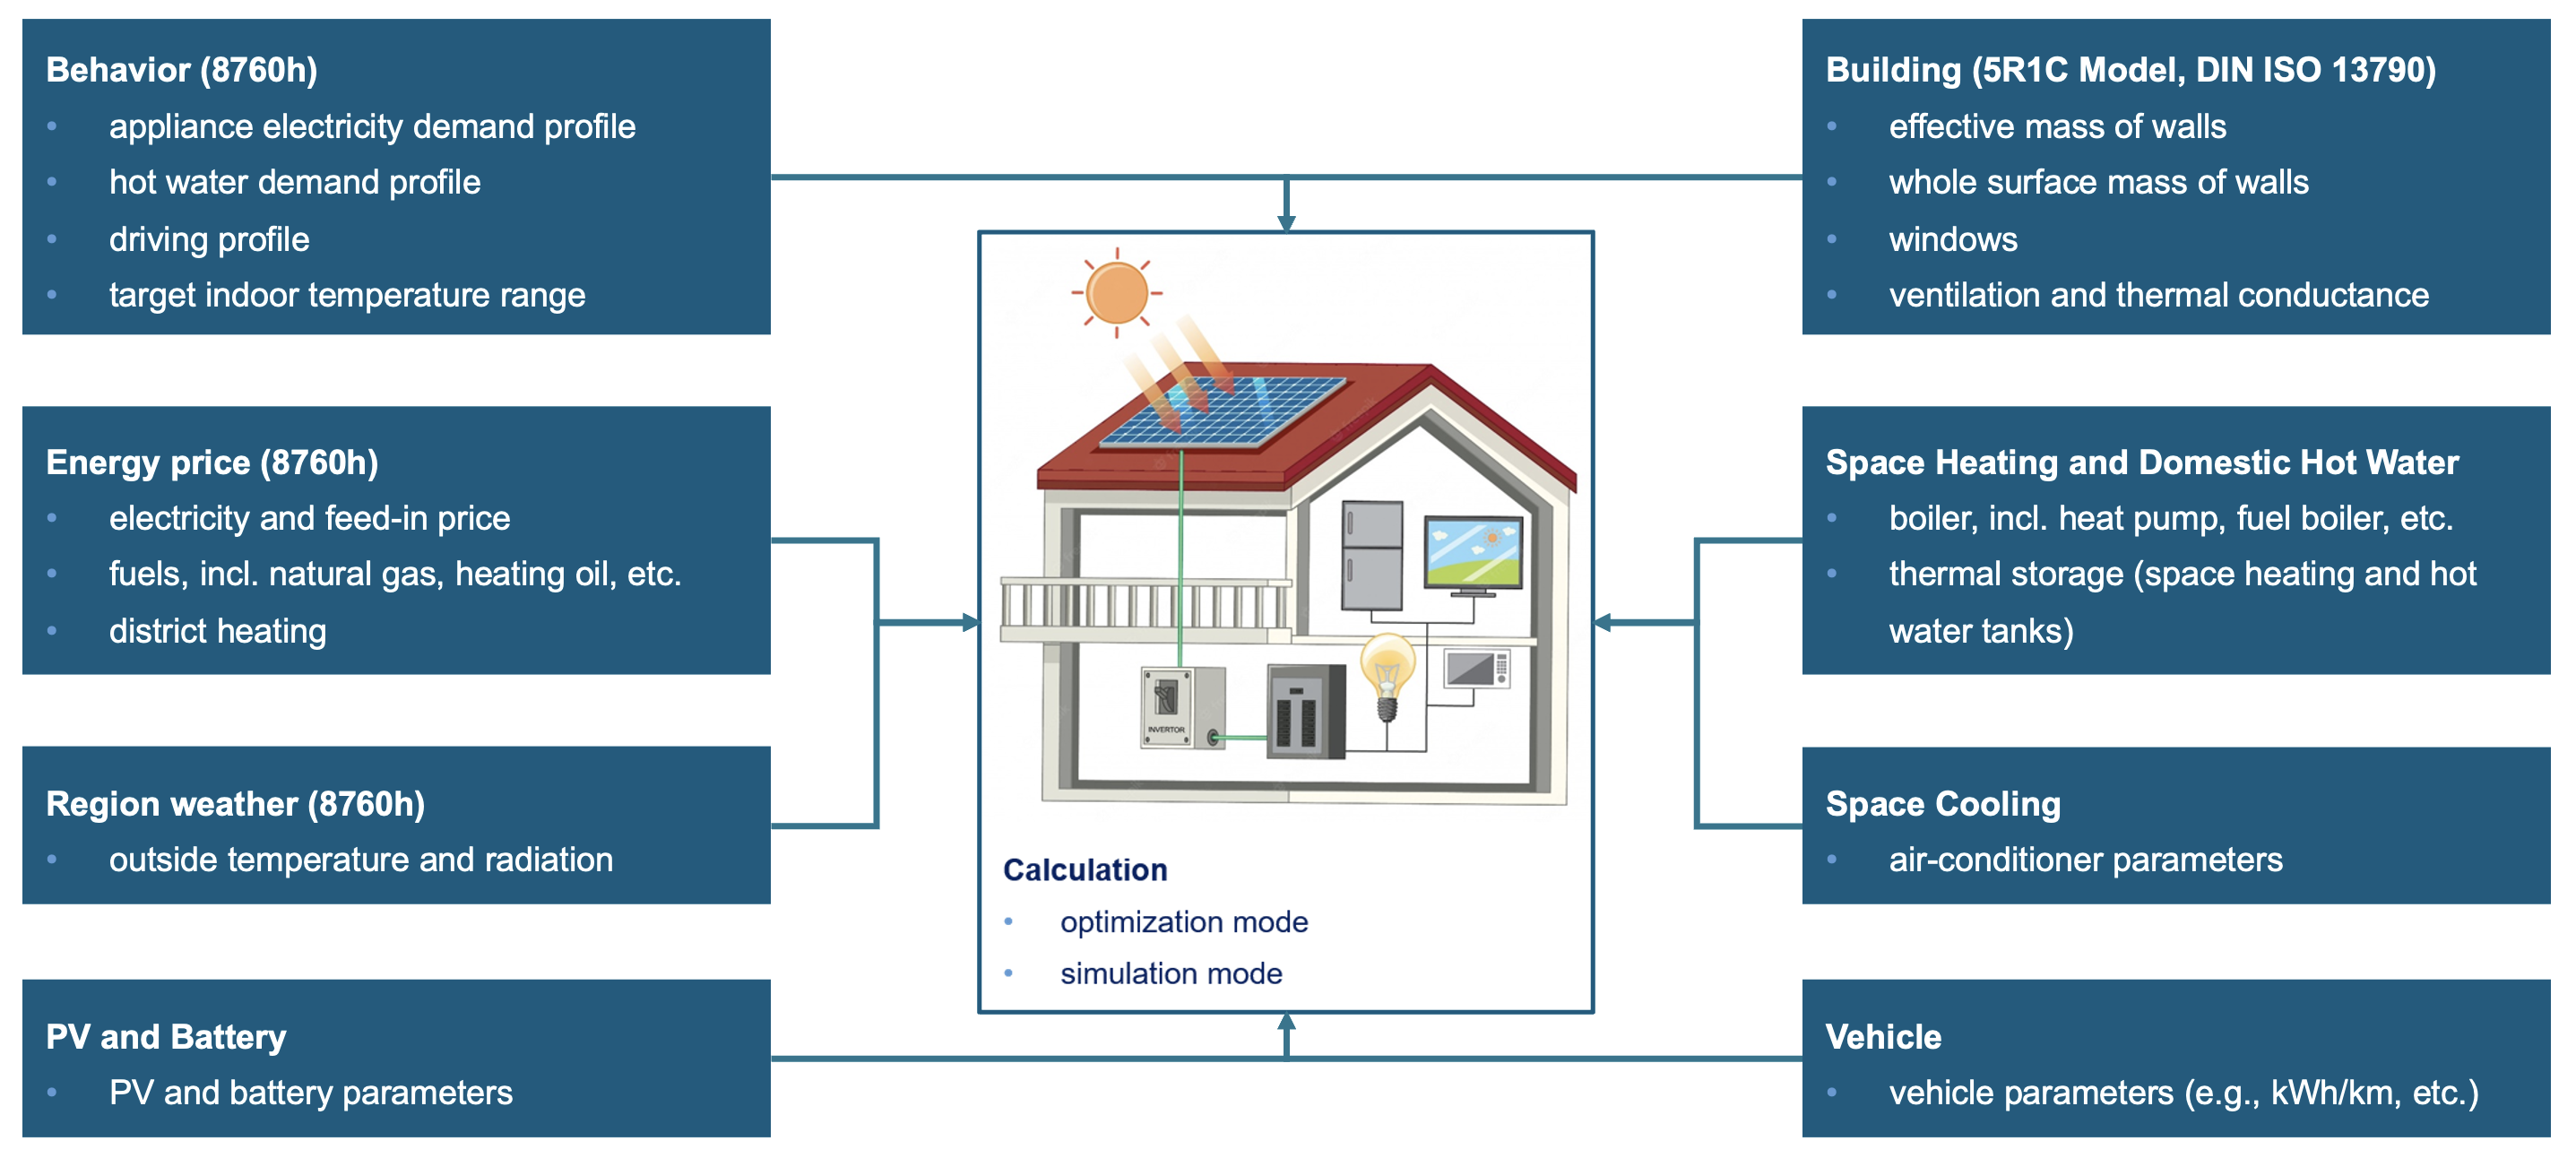
\includegraphics[width=\textwidth]{Images/flex-operation.png}
  \caption{Model structure for individual households}
  \label{fig:flex-operation}
\end{figure}

%Researchers believe new societal trends have the potential to shift energy demands between sectors and might reinforce or diminish one another when they occur at the same time \cite{2050}. 
%Researchers and organisations are paying increasing attention to how new societal trends are affecting energy demand.
%It is therefore important to access current and (foreseeable) future societal trends concerning the impact that they might have on future energy demand \cite{2050}. 

%Four arising societal trend clusters that are likely to shape future energy demand in European countries (and worldwide) were established by Brugger et al. \cite{2050}:  
%\emph{
%  (1) the digitalization of the economy and of private life; 
%  (2) new social and economic models, including the sharing economy and prosumaging (combination of producing, consuming and managing of energy); 
%  (3) industrial transformation, including decarbonization of industrial processes and the circular economy (including a stronger focus on material efficiency); 
%  (4) quality of life, including health effects, urbanization and regionalization. 
%}
%
%\begin{itemize}
%  \item \textbf{Digitalization of life} %\\ the digitalization of the economy and of private life;
%  \item \textbf{New social and economic models} %\\ including the sharing economy and prosumaging (combination of producing, consuming and managing of energy);
%  \item \textbf{Industrial transformation} %\\ including decarbonization of industrial processes and the circular economy (including a stronger focus on material efficiency);
%  \item \textbf{Quality of life} %\\ including health effects, urbanization and regionalization. 
%\end{itemize}
%
%The newTRENDs project develops the analytical basis for a “2050 Energy Efficiency Vision” by considering new societal trends in energy demand modeling \cite{newtrends}. 
%Considering the impact of these new societal trends on energy demand from a closer sectoral perspective,
%Yu et al. \cite{newtrends} identified four energy sectors: 
%
%\begin{itemize}
%  \item industry, 
%  \item transport,  
%  \item tertiary, 
%  \item residential.  
%\end{itemize}

%This proposed thesis will focus on the residential sector while taking scenarios of “consumers” becoming “prosumers” (with \gls{pv}) and “prosumagers” (adding energy storage and \gls{sems}) \cite{consumer} into account.  



%\subsubsection{The FLEX-Behaviour model}

%The FLEX-Behaviour model \cite{newtrends} facilitates the modeling of household behavior, including activity profiles and corresponding load profiles. 
%By generating an hourly activity and energy demand profile for a pre-defined household, this model provides a comprehensive assessment of the energy consumption patterns of an individual household.
%
%The estimates generated by the FLEX-Behaviour model refer to: 
%\begin{itemize}
%  \item appliance electricity demand,
%  \item domestic hot water demand,
%  \item driving profile, and
%  \item building occupation.
%\end{itemize}

%\subsubsection{INVERT/EE-Lab and FORECAST-Appliance}
%
%INVERT/EE-Lab and FORECAST-Appliance are the two models that can cover the energy consumption of residential buildings. The two models complement each other and cover the total energy consumption of households. 
%However, both INVERT/EE-Lab and FORECAST-Appliance calculate the energy consumption at the annual resolution and cannot model the prosumaging behavior and energy community, which requires an hourly resolution to consider the impact of household behavior, \gls{pv} generation, and energy storage (thermal and battery) on energy consumption. 
%In this regard, the FLEX-Operation and FLEX-Community models were developed to improve the building modeling suite and support relevant policy analysis \cite{newtrends}. 

%\subsubsection{FLEX-Community}
%
%FLEX-Community models the operation of an energy community, i.e., household interaction, aggregator optimisation. 
%It can be applied to support the aggregators designing and evaluating business models, as well as making investment decisions, for example, the self-owned battery, \gls{pv} panels, etc. \cite{newtrends}.


%\section{Recommender systems}
%
%Recommender systems (\gls{rs}) typically refer to software programs that furnish personalised suggestions of products, services, or content to users. 
%These systems employ different methods and algorithms to produce recommendations and are commonly implemented across different domains. 
%
%Kirsten Swearingen and Rashmi Sinha's research \cite{rs} suggests that an effective recommender system is perceived by users as a trustworthy system that can be relied upon. 
%To enable trust in an \gls{rs}, they recommend implementing the following measures:
%\emph{
%  having transparent system logic; 
%  suggesting novel items; 
%  offering comprehensive information about recommended items; 
%  and enabling users to refine their recommendations by specifying preferred or excluded genres.
%}